
\topmargin 0.0cm
\oddsidemargin 0.2cm
\textwidth 16cm 
\textheight 21cm
\footskip 1.0cm

\newcommand{\parfrac}[2]{\left( \frac{#1}{#2} \right)}
\newcommand{\lami}[1]{\lambda_{#1}}

\captionsetup[figure]{labelfont={bf}, labelsep=period, name={Fig.}}
\captionsetup[table]{labelfont={bf}, labelsep=period, name={Table}}
\renewcommand\thefigure{S\arabic{figure}}
\renewcommand\thetable{S\arabic{table}}
\renewcommand\theequation{S\arabic{equation}}

\setcounter{figure}{0}
\setcounter{equation}{0}
\setcounter{page}{1}

\title{ {\Large Supplementary Materials for} \\
{\large \textbf{Membrane heterogeneity alters our interpretation of effective energy barriers to transport}} \\
{\normalsize Nathanael S. Schwindt \textit{et al.}} \\
{\small $^\ast$Corresponding author. Email: michael.shirts@colorado.edu} }

\author{}
\date{}

\baselineskip24pt
\maketitle

\noindent \textbf{This PDF file includes:}

\begin{itemize}[noitemsep]
    \item[] Supplementary Text
    \item[] Figs. S1 to S5
    \item[] Table S1 to S2
    \item[] References (46 to 50)
\end{itemize}

\clearpage
\pagebreak

\section*{Supplementary Text}

\underline{Previous theoretical framework} \\
The original derivation by Zwolinski and coworkers~\cite{zwolinski_diffusion_1949} modeled membrane flux in terms of point-to-point jumps of molecules governed by rate constants. Thus, the net flux ($Q$) between equilibrium positions within the membrane becomes the difference in the forward and backward molecular jump rates through a cross-sectional area. A single barrier with equal forward and backward rate constants ($k$) and jump lengths ($\lambda$) leads to Fick's first law of diffusion (Eq.~\ref{eq:SM_ficks_law}) with diffusion coefficient $D = k\lambda^2$.

\begin{equation}
    Q = -D \frac{\text{d}C}{\text{d}x}
    \label{eq:SM_ficks_law}
\end{equation}

At steady state, the flux is a set of rate equations relating all local equilibrium positions along the direction of transport. Assuming a constant flux across the membrane and eliminating all the local concentrations gives an expression for the flux in terms of the local rate constants $k_i$, jump lengths $\lami{i}$, and initial $C_0$ and final $C_{m+1}$ concentrations shown in Eq.~\ref{eq:SM_flux1}, where $n$ is the total number of jumps along the transport coordinate.

\begin{equation}
    Q = \frac{ \displaystyle k_0 \lami{0} C_0 - \prod_{i=1}^n \parfrac{k_i' \lami{i}'}{k_i \lami{i}} k_{n+1}' \lami{n+1}' C_{n+1} } { \displaystyle 1 +  \sum_{r=1}^n \prod_{i=1}^r \parfrac{k_i' \lami{i}'}{k_i \lami{i}} }
    \label{eq:SM_flux1}
\end{equation}

\noindent Under transition state theory, the individual rate constants $k_i$ can be related to free energy barriers $\Delta G^{\ddagger}_i$ by 

\begin{equation}
    k_i = \kappa_i \frac{k_B T}{h} \exp{\parfrac{-\Delta G^{\ddagger}_i}{R T}}
    \label{eq:SM_TST_rate_constant1}
\end{equation}

\noindent $\kappa_i$ is the transmission coefficient (generally assumed to be unity for membrane processes), and $k_B$, $T$, and $h$ are Boltzmann's constant, temperature, and Planck's constant, respectively. Zwolinski et al.~\cite{zwolinski_diffusion_1949} and later del Castillo et al.~\cite{del_castillo_energy-barrier_1979} expanded the expression for flux in terms of free energy barriers to include external forces. Here, we explore the model without external forces, as external forces will only increase or decrease the free energy barriers without impacting the behavior of the model. 

Zwolinksi and coworkers verified their model on biological membranes using a simple setup with four distinct rate constants for the solution $k_s$, the solution-membrane interface $k_{sm}$, the membrane $k_M$, and the membrane-solution interface $k_{ms}$. The authors evaluated Eq.~\ref{eq:SM_flux1} for the solution-membrane-solution scenario under the assumptions that all jump lengths are equal, all free energy barriers within the membrane are equal, and diffusion within the membrane is the dominating step. They arrived at the following equation for membrane permeability ($P$)

\begin{equation}
    P = \frac{k_{sm} k_M \lambda}{m k_{ms}}
\end{equation}

\noindent As a result, they expressed membrane permeability in terms of a single, effective free energy barrier that includes the solution-membrane, membrane, and membrane-solution barriers. They claimed that this effective free energy barrier represents the difference in free energy between the species in solution and the species at the top of the highest potential energy barrier within the membrane. They extracted the enthalpic ($\Delta H_{eff}^{\ddagger}$) and entropic ($\Delta S_{eff}^{\ddagger}$) contributions to permeability from the Gibbs-Helmholtz relation. 

\begin{eqnarray}
    P &=& \parfrac{\lambda^2}{\delta} \parfrac{k_B T}{h} \exp{\parfrac{-\Delta G_{eff}^{\ddagger}}{R T}} \nonumber \\ 
    &=& \parfrac{\lambda^2}{\delta} \parfrac{k_B T}{h} \exp{\parfrac{\Delta S_{eff}^{\ddagger}}{R}} \exp{\parfrac{-\Delta H_{eff}^{\ddagger}}{R T}}
    \label{eq:SM_P_eyring1949}
\end{eqnarray}

$\delta$ in Eq.~\ref{eq:SM_P_eyring1949} is the membrane thickness, defined as $\delta = m\lambda$. This expression has been applied to both biological and polymeric membrane systems as a way to explore the molecular mechanisms governing membrane permeability~\cite{lopez_enthalpic_2017,shefer_enthalpic_2021,shefer_applying_2022}.

Giddings and Eyring also explored barrier kinetics primarily through the lens of nucleation~\cite{giddings_multi-barrier_1958}. Starting from Eq.~\ref{eq:SM_flux1}, the authors represented the effective free energy barrier for flux in terms of the individual point-to-point rate constants. While they did not explicitly state the similarity, the effective free energy barrier is in the form of multiple parallel resistances (see Equation 7 in reference~\cite{giddings_multi-barrier_1958}). They developed a “kT-cutoff model” to identify the non-negligible barriers (i.e. those within $k_B T$ of the maximum barrier). They concluded that for a series of jumps over unequal free energy barriers, the highest barrier does not define the overall flux but rather contributes the most to a sum of non-negligible barriers. Furthermore, they showed that the effective barrier depends only on the magnitude of the contributing barriers, not on their order. 

Scheuplein further explored the idea that position does not matter in his analysis of Gidding and Eyring’s multibarrier kinetics model more specifically applied to membrane permeability~\cite{scheuplein_application_1968}. Scheuplein grouped membrane barriers of similar size and represented membrane transport across many unequal groups as transport across a series of membranes with equal barriers. For barrier groups $\alpha, \beta, ..., \omega$, the permeability becomes 

\begin{equation}
    \frac{1}{P} = \parfrac{m}{\lambda} \sum_{i=\alpha}^{\omega} \parfrac{p_i}{K_{si} k_i}
\end{equation}

\noindent $m$ is the total number of barriers, $K_{si}$ is the partition coefficient from the solution to the $i^{th}$ minimum in the membrane, and $p_i$ is the probability of occurrence of the $i^{th}$ kind of barrier. This representation shows that the permeability is dependent on the individual probabilities and rate constants within the membrane. Therefore, the permeability is most affected by the highest and the most probable membrane barriers. 

This equation leads to interpreting membrane permeability as combining parallel resistances. Wendt et al.~derived a similar interpretation of permeability for pores in series~\cite{wendt_effect_1976}, and del Castillo et al.~explicitly showed how the multibarrier kinetic model can be thought of under this context~\cite{del_castillo_energy-barrier_1979}. Wendt and coworkers' primary assumptions were that transport can be treated as one-dimensional and that there is no internal concentration polarization within the membrane. From these assumptions, they showed that the overall flux in a series of non-sieving pores is equivalent to flux through a single pore with an overall permeability in the form of parallel resistances. Expanding to an array of pores, they showed that the overall flux in parallel pores is a sum of the individual pore fluxes. The overall permeability for the parallel array of pores is the area-weighted sum of the $n$ individual pore permeabilities ($P_i$) as shown in Eq.~\ref{eq:SM_parallel_permeability}. 
\begin{equation}
    P = \sum_{i=1}^n \frac{A_i}{A_0} P_i
    \label{eq:SM_parallel_permeability}
\end{equation}

\noindent where $A_i$ is the individual pore area and $A_0$ is the total membrane area considered, generally assumed to be a unit area. The individual pore areas are not required to sum to the total area. As a result, the overall permeability $P$ describes transport through the accessible area. If the pore areas do sum to the total area, the overall permeability becomes a weighted average, and the entire  membrane area is accessible for transport. del Castillo et al.~also explored these permeability expressions under arbitrary external forces, arguing that the overall flux depends on the distribution of parallel permeabilities, but in most cases, it will be near the pure diffusion limit. Additionally, they provided a weak constraint on the applicability of the multibarrier kinetic model for membrane transport. \\

\noindent \underline{Derivation of the permeability with distributions of barriers, jumps, and paths} \\
To construct our framework, we start with the main assumptions of Eyring's multibarrier kinetic model, and then relax some of these assumptions. Their assumptions were: 
\begin{enumerate}
    \item steady state flux can be represented by point-to-point molecular jumps between locally equilibrated states,
    \item membrane transport is one-dimensional in the solution-membrane-solution framework,
    \item an aqueous solution is diffusing through the membrane, and membrane diffusion is the primary hindrance to transport,
    \item the transmission coefficient is one for all rate constants,
    \item the free energy barriers within the membrane are a series of equal free energy barriers, and 
    \item the jump lengths between local barriers are equal.
\end{enumerate}

We start with Eq.~\ref{eq:SM_flux2}~\cite{zwolinski_diffusion_1949} and relax the assumptions that the free energy barriers within the membrane are a series of equal free energy barriers and the jump lengths between local barriers are equal.

\begin{equation}
    Q = \frac{ \displaystyle k_0 \lami{0} C_0 - \prod_{i=1}^n \parfrac{k_i' \lami{i}'}{k_i \lami{i}} k_{n+1}' \lami{n+1}' C_{n+1} } { \displaystyle 1 +  \sum_{r=1}^n \prod_{i=1}^r \parfrac{k_i' \lami{i}'}{k_i \lami{i}} }
    \label{eq:SM_flux2}
\end{equation}

\noindent As a result, the numerator expands to 

\begin{align*}
     & k_0 \lami{0} C_0 - \prod_{i=1}^n \parfrac{k_i' \lami{i}'}{k_i \lami{i}} k_{n+1}' \lami{n+1}' \lambda C_{n+1} \\
     &= k_s \lami{s} C_0 - \left[ \parfrac{k_s \lami{s}}{k_s \lami{s}} ... \parfrac{k_s \lami{s}}{k_s \lami{s}} \parfrac{k_s \lami{s}}{k_{sm} \lami{sm}} \parfrac{k_{ms} \lami{ms}}{k_{M,1} \lami{M,1}} \parfrac{k_{M,1} \lami{M,1}}{k_{M,2} \lami{M,2}} ... \right. \\
     & \hspace{60px} \left. \parfrac{k_{M,m-1} \lami{M,m-1}}{k_{M,m} \lami{M,m}} \parfrac{k_{M,m} \lami{M,m}}{k_{ms} \lami{ms}} \parfrac{k_{sm} \lami{sm}}{k_s \lami{s}} \parfrac{k_s \lami{s}}{k_s \lami{s}} ... \parfrac{k_s \lami{s}}{k_s \lami{s}} \right] k_s \lami{s} C_{n+1} \\
     &=  k_s \lami{s} C_0 - \left[ \parfrac{k_s \lami{s}}{k_s \lami{s}}^{s-1} \parfrac{k_s \lami{s}}{k_{sm} \lami{sm}} \parfrac{k_{ms} \lami{ms}}{k_{M,1} \lami{M,1}} \parfrac{k_{M,1} \lami{M,1}}{k_{M,2} \lami{M,2}} ... \right. \\
     & \hspace{60px} \left. \parfrac{k_{M,m-1} \lami{M,m-1}}{k_{M,m} \lami{M,m}} \parfrac{k_{M,m} \lami{M,m}}{k_{ms} \lami{ms}} \parfrac{k_{sm} \lami{sm}}{k_s \lami{s}} \parfrac{k_s \lami{s}}{k_s \lami{s}}^{s'-1} \right] k_s \lami{s} C_{n+1} \\
     &= k_s \lami{s} C_0 - \left( 1 \right) k_s \lami{s} C_{n+1}
\end{align*}

\pagebreak

\noindent The denominator expands to 

\begin{align*}
    & 1 + \sum_{r=1}^n \prod_{i=1}^r \parfrac{k_i' \lami{i}'}{k_i \lami{i}} \\
    &= 1 + \left( s-1 \right) \left[ \parfrac{k_s \lami{s}}{k_s \lami{s}}^{s-1} \right]_{s-1} + \left[ \parfrac{k_s \lami{s}}{k_s \lami{s}}^{s-1} \parfrac{k_s \lami{s}}{k_{sm \lami{sm}}} \right]_{s} \\
    & \hspace{20px} + \left[ \parfrac{k_s \lami{s}}{k_s \lami{s}}^s \parfrac{k_s \lami{s}}{k_{sm } \lami{sm}} \parfrac{k_{ms} \lami{ms}}{k_{M,1} \lami{M,1}} \right]_{s+1} \\
    & \hspace{20px} + \left[ \parfrac{k_s \lami{s}}{k_s \lami{s}}^{s-1} \parfrac{k_s \lami{s}}{k_{sm} \lami{sm}} \parfrac{k_{ms} \lami{ms}}{k_{M,1} \lami{M,1}} \parfrac{k_{M,1} \lami{M,1}}{k_{M,2} \lami{M,2}} \right]_{s+2} \\ 
    & \hspace{20px} + ... + \left[ \parfrac{k_s \lami{s}}{k_s \lami{s}}^{s-1} \parfrac{k_s \lami{s}}{k_{sm} \lami{sm}} \parfrac{k_{ms} \lami{ms}}{k_{M,1} \lami{M,1}} \parfrac{k_{M,1} \lami{M,1}}{k_{M,2} \lami{M,2}} ... \right. \\
    & \hspace{65px} \left. \parfrac{k_{M,m-1} \lami{M,m-1}}{k_{M,m} \lami{M,m}} \parfrac{k_{M,m} \lami{M,m}}{k_{ms} \lami{ms}} \right]_{s+m+1} \\
    & \hspace{20px} + \left[ \parfrac{k_s \lami{s}}{k_s \lami{s}}^{s-1} \parfrac{k_s \lami{s}}{k_{sm} \lami{sm}} \parfrac{k_{ms} \lami{ms}}{k_{M,1} \lami{M,1}} \parfrac{k_{M,1} \lami{M,1}}{k_{M,2} \lami{M,2}} ... \right. \\
    & \hspace{40px} \left. \parfrac{k_{M,m-1} \lami{M,m-1}}{k_{M,m} \lami{M,m}} \parfrac{k_{M,m} \lami{M,m}}{k_{ms} \lami{ms}} \parfrac{k_{sm} \lami{sm}}{k_s \lami{s}} \right]_{s+m+2} \\
    & \hspace{20px} + \left( s'-1 \right) \left[ \parfrac{k_s \lami{s}}{k_s \lami{s}}^{s-1} \parfrac{k_s \lami{s}}{k_{sm} \lami{sm}} \parfrac{k_{ms} \lami{ms}}{k_{M,1} \lami{M,1}} \parfrac{k_{M,1} \lami{M,1}}{k_{M,2} \lami{M,2}} ... \right. \\
    & \hspace{80px} \left. \parfrac{k_{M,m-1} \lami{M,m-1}}{k_{M,m} \lami{M,m}} \parfrac{k_{M,m} \lami{M,m}}{k_{ms} \lami{ms}} \parfrac{k_{sm} \lami{sm}}{k_s \lami{s}} \parfrac{k_s \lami{s}}{k_s \lami{s}}^{s'-1} \right]_{s+m+s'+1} \\
    &= 1 + \left( s-1 \right) + \parfrac{k_s \lami{s}}{k_{sm} \lami{sm}} + \parfrac{k_s \lami{s} k_{ms} \lami{ms}}{k_{sm} \lami{sm} k_{M,1} \lami{M,1}} + \parfrac{k_s \lami{s} k_{ms} \lami{ms}}{k_{sm} \lami{sm} k_{M,2} \lami{M,2}} + ... \\
    & \hspace{20px} + \parfrac{k_s \lami{s} k_{ms} \lami{ms}}{k_{sm} \lami{sm} k_{M,m} \lami{M,m}} + \parfrac{k_s \lami{s}}{k_{sm} \lami{sm}} + 1 + \left( s'-1 \right) \\
    &= s + s' + 2 \parfrac{k_s \lami{s}}{k_{sm} \lami{sm}} + \parfrac{k_s \lami{s} k_{ms} \lami{ms}}{k_{sm} \lami{sm}} \sum_{j=1}^m \parfrac{1}{k_{M,j} \lami{M,j}}
\end{align*}

\noindent where the subscripts on bracketed terms track the sum over all jumps. Eq.~\ref{eq:SM_flux2} simplifies to

\begin{equation}
    Q = \frac{k_s \lami{s} \left( C_0 - C_{n+1} \right)}{\displaystyle s + s' + 2 \parfrac{k_s \lami{s}}{k_{sm} \lami{sm}} + \parfrac{k_s \lami{s} k_{ms} \lami{ms}}{k_{sm} \lami{sm}} \sum_{j=1}^m \parfrac{1}{k_{M,j} \lami{M,j}}}
    \label{eq:SM_flux_final}
\end{equation}

\noindent Therefore, the permeability becomes

\begin{equation}
    P = \frac{1}{\displaystyle \parfrac{s}{k_s \lami{s}} + \parfrac{s'}{k_s \lami{s}} + \parfrac{2}{k_{sm} \lami{sm}} + \parfrac{k_{ms} \lami{ms}}{k_{sm} \lami{sm}} \sum_{j=1}^m \parfrac{1}{k_{M,j} \lami{M,j}}}
\end{equation}

\noindent In membrane transport, the jump rates through solution ($k_s$) are significantly larger than those through the membrane interface and the bulk membrane. As a result, the permeability can be expressed only in terms of the interfacial and membrane rate constants as shown in Eq.~\ref{eq:SM_permeability_rates}.

\begin{equation}
    \frac{1}{P} = \parfrac{2}{k_{sm} \lami{sm}} + \parfrac{k_{ms} \lami{ms}}{k_{sm} \lami{sm}} \sum_{j=1}^m \parfrac{1}{k_{M,j} \lambda_{M,j}}
    \label{eq:SM_permeability_rates}
\end{equation}

\noindent The first term in Eq.~\ref{eq:SM_permeability_rates} is associated with diffusion through the solution-membrane interface, and the second term is associated with diffusion through the membrane. For most polymeric membranes, the rate-determining step is diffusion through the membrane, so Eq.~\ref{eq:SM_permeability_rates} can be approximated with only the second term. The resulting expression for permeability in terms of the rate constants for transport is shown in Eq.~\ref{eq:SM_membrane_diffusion_limited_permeability}.

\begin{equation}
    P = \frac{k_{sm} \lami{sm}}{\displaystyle k_{ms} \lami{ms} \sum_{j=1}^m \parfrac{1}{k_{M,j} \lambda_{M,j}}}
    \label{eq:SM_membrane_diffusion_limited_permeability}
\end{equation}

\noindent Under transition state theory, the individual rate constants $k_i$ can be related to free energy barriers $\Delta G^{\ddagger}_i$ by 

\begin{equation}
    k_i = \kappa_i \frac{k_B T}{h} \exp{\parfrac{-\Delta G^{\ddagger}_i}{k_B T}}
    \label{eq:SM_TST_rate_constant2}
\end{equation}

\noindent Relating Eq.~\ref{eq:SM_membrane_diffusion_limited_permeability} to the associated free energy barriers with Eq.~\ref{eq:SM_TST_rate_constant2} yields Eq.~\ref{eq:SM_permeability_barriers} for permeability across a series of unequal membrane barriers in terms of the free energy barriers at transition $\Delta G_j^{\ddagger}$.

\begin{equation}
    P = \frac{\displaystyle \parfrac{\lambda_{sm}}{\lambda_{ms}} \parfrac{k_B T}{h} \exp{\parfrac{ -\left( \Delta G_{sm}^{\ddagger} - \Delta G_{ms}^{\ddagger} \right)}{R T}}}{\displaystyle \sum_{j=1}^m \parfrac{1}{\lambda_{M,j} \exp{\parfrac{-\Delta G_{M,j}^{\ddagger}}{R T}}}}
    \label{eq:SM_permeability_barriers}
\end{equation} \\

\noindent \underline{Derivation of the effective free energy barrier} \\
Zwolinski and coworkers express the effective free energy barrier to permeability as 

\begin{eqnarray}
    P &=& \parfrac{\lambda^2}{\delta} \parfrac{k_B T}{h} \exp{\parfrac{-\Delta G_{eff}^{\ddagger}}{R T}} \nonumber \\ 
    &=& \parfrac{\lambda^2}{\delta} \parfrac{k_B T}{h} \exp{\parfrac{\Delta S_{eff}^{\ddagger}}{R}} \exp{\parfrac{-\Delta H_{eff}^{\ddagger}}{R T}}
    \label{eq:SM_permeability_eyring1949}
\end{eqnarray}

\noindent We incorporate parallel molecular pathways and distributions of membrane jumps and barriers into the transition-state theory model for membrane permeability, as shown in Eq.~\ref{eq:SM_overall_permeability}.

\begin{equation}
    P = \sum_{i=1}^{n} \left[ \frac{\displaystyle \parfrac{A_i}{A_0} \parfrac{\lambda_{sm}}{\lambda_{ms}} \parfrac{k_B T}{h} \exp{\parfrac{ -\left( \Delta G_{sm}^{\ddagger} - \Delta G_{ms}^{\ddagger} \right)}{R T}}}{\displaystyle \sum_{j=1}^{m_i} \parfrac{1}{\lambda_{M,i,j} \exp{\parfrac{-\Delta G_{M,i,j}^{\ddagger}}{R T}}}} \right]
    \label{eq:SM_overall_permeability}
\end{equation}

\noindent We equate these expressions for permeability and solve for the effective free energy barrier in terms of the distributions of membrane barriers and parallel paths. 

% insert step-by-step solve 

\begin{equation}
    \Delta G_{eff}^{\ddagger} = -R T \ln{\left[ \sum_{i=1}^{n} \frac{ \displaystyle \parfrac{A_i}{A_0} \parfrac{\delta}{\lami{avg}^2} \parfrac{\lambda_{sm}}{\lambda_{ms}} }{\displaystyle \sum_{j=1}^{m_i} \parfrac{1}{\lambda_{M,i,j}} \exp{\parfrac{\Delta G_{M,i,j}^{\ddagger}}{R T}}} \right]} + \left( \Delta G_{sm}^{\ddagger} - \Delta G_{ms}^{\ddagger}\right)
    \label{eq:SM_effective_barrier}
\end{equation} \\

\noindent \underline{Estimating the number of paths per unit area} \\
We estimate the number of paths per unit area for the polyamide membrane to be an order of magnitude fewer than what is expected for single-walled carbon nanotubes (SWCNT). SWCNT with diameter 1.7~nm have been reported to pack with density \num{1.9e12} paths per \unit{\cm\squared}~\cite{jue_ultrapermeable_2020}. If all the area is occupied by circular nanotubes with diameter 1.7~nm and negligible thickness, the theoretical packing density is \num{4.4e13} paths per \unit{\cm\squared}. We use this ratio of actual packing density to theoretical packing density to approximate the actual packing density of SWCNT with diameter 0.5~nm, the reported average pore size for polyamide membranes~\cite{chu_variation_2021, wang_water_2023}. 

\begin{equation}
    \left( \frac{\text{actual, } d=1.7 \unit{\nm}}{\text{theoretical, } d=1.7 \unit{\nm}} \right) \times \left( \text{theoretical, } d=0.5 \unit{\nm} \right) = \left( \text{actual, } d=0.5 \unit{\nm} \right)
\end{equation}

\noindent We estimate the actual packing density of SWCNT with diameter 0.5~nm to be \num{2.2e13} paths per \unit{\cm\squared} or 0.22 paths per \unit{\nm\squared}. Therefore, we estimate the actual number of paths per unit area for polyamide membranes to be 0.022 paths per \unit{\nm\squared}. The results we present consider a total unit area of 0.1 \unit{\um\squared}, or \num{1.0e7} $\text{\AA}^2$, and a single path area of $\pi (5 \text{\AA})^2 = 19.635~\text{\AA}^2$. These areas correspond to 2196 paths per 0.1 \unit{\um\squared}. \\

\noindent \underline{Effect of jump distributions on the effective free energy barrier} \\
Given a fixed membrane thickness, the distribution of number of jumps and the length of jumps are directly related. Thus, we can examine the effects of only the distribution in the number of jumps for a given membrane thickness. We choose a physically realistic membrane thickness and hold all membrane free energy barriers equal. We draw the number of jumps from a (truncated) normal distribution because we can change the variance while maintaining a physically relevant mean. For this analysis, we model 5000 paths through a membrane of thickness 400 \AA. We set the mean number of jumps to be 100, and we adjust the jump length to ensure the membrane thickness remains constant. We vary the standard deviation in the number of jumps between 5 and 200. Because this can result in a negative number of jumps, we redraw each negative draw from a normal distribution until no paths have a non-positive number of jumps. This results in a nearly normal distribution for large variances, but a truncated distribution at $N=1$ and below for larger variances. 

We find that the effective free energy barrier decreases with increasing variance in the number of jumps, but the change is significantly less than the effects from distributions of barrier heights in all physical scenarios. Fig.~\ref{fig:jump_variances} shows the relationship between the effective free energy barrier and the standard deviation in number of jumps. 

The effective barrier decreases negligibly when the variance is small. When the variance becomes larger, a small number of paths have very few jumps, which results in moderately decreased effective barrier, up to 1.5 kcal/mol. The barrier decreases negligibly again for larger standard deviations of the truncated distribution, when the number of paths with $N=1$ barriers predominates. In contrast, modest variance in the barrier height distribution, as shown by the normally distributed barrier heights in Fig.~3B in the main text, changes the effective barrier by 5.3 kcal/mol.

At large standard deviation, the effective barrier becomes dominated by paths with only a few jumps. Fig.~\ref{fig:perm_percentage}A confirms this trend by showing the percentage of the total permeability through each path for the highest variance distribution (standard deviation 200). Conversely, when all paths have nearly the same number of jumps, the permeability is evenly distributed across the paths, as shown in Fig.~\ref{fig:perm_percentage}B. The standard deviation in the number of jumps for Fig.~\ref{fig:perm_percentage}B is 5. 

Physically, larger jumps along the transport coordinate with the approximately the same membrane thickness reduce the number of barriers the molecules must cross. Jump lengths affect the single path permeability as a sum of reciprocal jump lengths, so small jumps contribute more than large jumps. The distributions of jump lengths introduce some smaller jumps that drive the permeability lower and the effective free energy barrier higher. Individual jump lengths are likely to be correlated with their associated free energy barrier. However, the exponential contribution of the free energy barriers will dominate the contribution from the jump lengths. For membranes with heterogeneity in their free energy barrier distributions, the variability of the smallest maximum barrier contributes significantly more than variability in the number and length of jumps through the membrane, and we thus focus primarily on the distribution of barrier heights in this study. \\

\noindent \underline{Accounting for concentration polarization in the membrane} \\
Previously reported barriers for NF and RO membranes range from 0 to $\sim$17 kcal/mol with most values lie between $\sim$4 and $\sim$8 kcal/mol~\cite{epsztein_towards_2020}. However, most of the reported values in the literature are likely an overestimation of the real barriers, as these values were measured without accounting for the increasing concentration polarization of the transported solutes with temperature. This phenomenon leads to higher concentration gradient over the membrane (and therefore higher driving force) with temperature, resulting in an increased solute flux that is not related to intrinsic activation (i.e., a permeability increase with temperature). Our measurements rigorously accounted for concentration polarization and therefore reflect more reliably the intrinsic barriers. 

In brief, to account for concentration polarization during the measurement of the permeability at the different temperatures, evaluation of the salt concentration on the membrane surface, $C_m$, was performed at each temperature by retrieving the mass transfer coefficient in the boundary layer, $k$, using the following correlation for the Sherwood number based on laminar (Eq.~\ref{eq:sherwood_laminar}) and turbulent (Eq.~\ref{eq:sherwood_turbulent}) flows in a rectangular channel without a spacer~\cite{mulder_basic_1996}: 
\begin{equation}
    \text{Sh} = 1.85 \left( \text{Re} \text{Sc} \frac{d_h}{L} \right)^{0.33}
    \label{eq:sherwood_laminar}
\end{equation}
\begin{equation}
    \text{Sh} = 0.04 \text{Re}^{0.75} \text{Sc}^{0.33}
    \label{eq:sherwood_turbulent}
\end{equation}
where Sh is the Sherwood number $\left( \text{Sh}=\left( \frac{k d_h}{D} \right) \right)$, Re is the Reynolds number ($\sim$3295 in our system), Sc is the Schmidt number $\left( \text{Sc} = \frac{\nu}{D} \right)$, where $D$ is the diffusion coefficient and $\nu$ is the kinematic viscosity), $d_h$ is the hydraulic radius (\num{1.55e-3}~m in our system), and $L$ is the cell length (0.06~m in our system). The height and width of the flow channel in our system were 0.8~mm and 25~mm, respectively. Because Re was in the borderline of laminar and turbulent flow in our system, we examined both the laminar and turbulent correlations. The diffusion coefficients of the different ions at the tested temperatures were calculated with the Stokes-Einstein equation using Stokes radii (Table~\ref{tab:stokes}). For each salt, the diffusion coefficient of the slower ion was used for the calculations of the Sherwood number. The evaluated $k$ values were then used in the film theory equation (Eq.~\ref{eq:film_theory}) to measure $C_m$.
\begin{equation}
    \frac{C_m - C_p}{C_f - C_p} = \exp{\left( \frac{J_w}{k} \right)}
    \label{eq:film_theory}
\end{equation}
$C_p$ and $C_f$ are the salt concentrations in the permeate and the feed solution, respectively, $J_w$ is the permeate flux (L~m$^{-2}$~h$^{-1}$), and $k$ is the mass transfer coefficient (m~s$^{-1}$). \\

\noindent \underline{Comparing the Arrhenius plots and transition-state theory plots} \\
Energy barriers to permeability are often measured as Arrhenius barriers, and the effective parameters are determined as the slope and intercept of $\ln(P)$ vs $1/T$. However, this form neglects the temperature dependence of the prefactor that is explicitly stated in transition-state theory. The difficulty with the transition-state theory approach is the need for additional parameters, namely average jump length $\lambda$ and membrane thickness $\delta$ in Eq.~\ref{eq:SM_permeability_eyring_effective}, which are challenging to measure. 

\begin{equation}
    P = \parfrac{\lambda^2}{\delta} \parfrac{k_B T}{h} \exp{\parfrac{-\Delta G_{eff}^{\ddagger}}{R T}}
    \label{eq:SM_permeability_eyring_effective}
\end{equation}

We perform both linear fits, and we determine the goodness of fit is not significantly different between the models. The $R^2$ is 0.642 for the Arrhenius treatment and 0.569 for the transition-state theory treatment. In Fig.~\ref{fig:arrhenius_vs_tst}, we show the linear fits for $\ln(P)$ and $\ln(P/T)$ for NaCl in the NF270 membrane. Table~\ref{tab:effective_enthalpies} shows the effective enthalpic barriers for each linearization. The errors shown are the standard errors in the slope parameter for the linear fit propagated to the effective enthalpic barrier. All the enthalpic barriers from transition state theory are within the mutual margin of error of the effective activation energies from Arrhenius theory. 

More importantly, the trends are completely preserved between the two approaches. Effective enthalpic barriers are 0.5 to 0.6 lower in the transition state theory versus Arrhenius theory in all cases, with the variation within 0.1, much smaller than the error. 

\clearpage
\pagebreak

% Figure S1 - effective barrier convergence
\begin{figure}[H]
    \centering
    \begin{subfigure}[b]{0.45\textwidth}
        \centering
        \includegraphics[width=\textwidth]{figures/effective_barrier_convergence_norm.png}
        \caption{Normally distributed barriers}
        \label{fig:convergence_normal}
    \end{subfigure}
    \hfill
    \begin{subfigure}[b]{0.45\textwidth}
        \centering
        \includegraphics[width=\textwidth]{figures/effective_barrier_convergence_exp.png}
        \caption{Exponentially distributed barriers}
        \label{fig:convergence_exponential}
    \end{subfigure}
    \caption{\textbf{{Convergence testing to determine necessary number of paths.}} The effective free energy barrier converges for both normally and exponentially distributed barriers for the distribution variances used in this paper converges within summation over 2000 pathways. Barrier distributions with higher variance will take more pathways to converge. Black points are single realizations of calculated effective free energy barriers, and red points are effective free energy barriers averaged over all realizations. We calculate 100 realizations for each number of paths.}
    \label{fig:convergence}
\end{figure}

\clearpage
\pagebreak

% Figure S2 - variance in jump distributions
\begin{figure}[ht!]
    \centering
    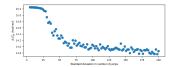
\includegraphics[width=\textwidth]{figures/figS2.pdf}
    \caption{\textbf{Effective barrier decreases with increasing variance in the number of jumps.} We show the overall effective free energy barrier as a function of the standard deviation for normally distributed numbers of jumps with mean 100. The jump length is adjusted to maintain a constant membrane thickness of 40 \AA. For each standard deviation, we calculate the overall effective free energy barrier over 5000 paths.}
    \label{fig:jump_variances}
\end{figure}

\clearpage
\pagebreak

% Figure S3 - percentage of permeability through paths
\begin{figure}[ht!]
    \centering
    \includegraphics[width=\textwidth]{figures/figS3.pdf}
    \caption{\textbf{Paths with only a few jumps contribute most to the permeability.} We calculate the percentage of the total permeability through paths with different numbers of jumps. The jump length is adjusted to maintain a constant membrane thickness of 40 \AA, and we calculate the overall effective free energy barrier over 5000 paths. (\textbf{A}) The standard deviation in the normally distributed number of jumps is 5, and the mean is 100. The permeability is evenly spread across paths, since all paths have similar number of jumps. (\textbf{B}) The standard deviation in the normally distributed number of jumps is 200, and the mean is 100. The permeability is dominated by paths with only a few jumps.}
    \label{fig:perm_percentage}
\end{figure}

\clearpage
\pagebreak

% Figure S4 - effective enthalpy for NaCl in water
\begin{figure}[ht!]
    \centering
    \includegraphics[width=0.75\textwidth]{figures/NaCl_in_water_TST.png}
    \caption{\textbf{Effective enthalpy for NaCl in water.} Linearized transition-state theory plot for the conductivity of NaCl in water, which corresponds to free diffusion of the ions. The least squares fit is shown as a line.}
    \label{fig:tst_NaCl_water}
\end{figure}

\clearpage
\pagebreak

% Figure S5 - Arrhenius vs TST
\begin{figure}[ht!]
    \centering
    \includegraphics[width=0.75\textwidth]{figures/TST_vs_Arrhenius_plots.png}
    \caption{\textbf{Comparison of transition-state theory and Arrhenius plots} Estimation of the effective enthalpic barriers from the transition-state theory model and the Arrhenius model are indistinguishable within error. Scatter points are the experimental data linearized to fit the corresponding model. The least squares fits are shown as lines. A 95\% confidence interval (shaded region) is provided with each least squares fit, determined by a nonparametric bootstrap over 1000 bootstraps.}
    \label{fig:arrhenius_vs_tst}
\end{figure}

\clearpage
\pagebreak

\begin{table}
    \centering
    \begin{tabular}{|c|c|c|}
        \hline
        System & Linearization & $E_a$ or $\Delta H_{eff}^{\ddagger}$ (kcal/mol) \\
        \hline
        \multirow{2}{*}{NaCl (NF270)} & $\ln (P)$   & $4.2 \pm 0.9$ \\\cline{2-3}
                                      & $\ln (P/T)$ & $3.6 \pm 0.9$ \\
        \hline
        \multirow{2}{*}{NaF (NF270)}  & $\ln (P)$   & $4.5 \pm 1.1$ \\\cline{2-3}
                                      & $\ln (P/T)$ & $3.9 \pm 1.1$ \\
        \hline
        \multirow{2}{*}{NaCl (RO)}    & $\ln (P)$   & $5.0 \pm 1.3$ \\\cline{2-3}
                                      & $\ln (P/T)$ & $4.5 \pm 1.3$ \\
        \hline
    \end{tabular}
    \caption{\textbf{Effective barriers from Arrhenius and transition-state theory models.} The activation parameter $E_a$ and the effective enthalpic barrier $\Delta H_{eff}^{\ddagger}$ are within their mutual margin of error for all systems.}
    \label{tab:effective_enthalpies} 
\end{table}

\clearpage
\pagebreak

\begin{table}
    \centering
    \begin{tabular}{|c|c|}
        \hline
         Species           & Stokes radius (nm)~\cite{nightingale_phenomenological_1959} \\
         \hline
         Sodium (Na$^+$)   & 0.184 \\ 
         \hline
         Fluoride (F$^-$)  & 0.166 \\
         \hline
         Chloride (Cl$^-$) & 0.121 \\
         \hline
    \end{tabular}
    \caption{\textbf{Stokes radii for the ions tested in the experimental filtration measurements.} All data is from reference~\cite{nightingale_phenomenological_1959}}
    \label{tab:stokes}
\end{table}